\newpage
{\bfseries ҒТАМР 31.15.37}
\hfill {\bfseries \href{https://doi.org/10.58805/kazutb.v.2.23-460}{https://doi.org/10.58805/kazutb.v.2.23-460}}

\sectionwithauthors{О.В. Рожкова, Ш.А. Мұздыбаева, А.Б. Бөкеева, С.Ж. Құдайбергенова,  В.И. Рожков, М.Т. Ермеков,  Ж.Т.Нұртай}{БЕНТОНИТ САЗЫН ТАУ-КЕН ӨНДІРІСІНІҢ ШАХТА СУЛАРЫН ТАЗАРТУДАҒЫ ҚОЛДАНУ ТИІМДІЛІГІ}

\begin{center}
{\bfseries \textsuperscript{1,3} О.В. Рожкова,\textsuperscript{2} Ш.А. Мұздыбаева, \textsuperscript{3}А.Б. Бөкеева, \textsuperscript{3}С.Ж. Құдайбергенова, \textsuperscript{3,4} В.И. Рожков, \textsuperscript{1}М.Т. Ермеков, \textsuperscript{5} Ж.Т.Нұртай}

\textsuperscript{1} «Science and Technology Solutions» АҚ, Алматы,
Қазақстан,

\textsuperscript{2}Халықаралық инженерлік-технологиялық университеті,
Алматы, Қазақстан,

\textsuperscript{3} КЕАҚ «С.Сейфуллин атындағы Қазақ агротехникалық
зерттеу университеті»,

Астана, Қазақстан,

\textsuperscript{4}«Алтай геологиялық-экологиялық институты» ЖШС,
Өскемен, Қазақстан,

\textsuperscript{5} «Қ.Құлажанов атындағы Қазақ технология және бизнес
университеті» АҚ, Астана, Қазақстан,

Корреспондент-автор: rozhkova.o@stsolutions.kz
\end{center}

Металлургиялық кәсіпорындардың ағынды суларын тазарту мақсатында
Шығыс-Қазақстан облысы Таған кен орнының бентониті зерттелген. Табиғи
сорбенттің және оның белсендірілген түрлерінің физика-химиялық
сипаттамаларын зерттеу үшін заманауи зерттеу әдістері қолданылған:
атомды-абсорбциялық спектрометрия, индуктивті байланысқан плазмамен
масс-спектрометрия, полярография және рентгенфлуоресцентті
спектрометрия, энергодисперсиондық талдау қосымшасымен электрондық
микроскопия. Бентониттің термиялық және термоқышқылдық белсендендірілуі
қарастырылған. Белсендендірілген формалардың құрылымы электрондық
микроскоп көмегімен анықталған. Табиғи және белсендендірілген түрлерінің
микроқұрылымдарын электрондық микроскоппен салыстыру кезінде құрылымының
ең көп өзгеруі термоқышқылдық белсендендіру кезінде жүргізілетінін
көрсетеді. Бентониттің кеуектілігі артып, беткі қабаты көбірек босайды.

Полиметалдық кен орнының ағынды суларын тазатру үшін бентониттің табиғи
және белсендендірілген түрлері қолданылған. Осы кезде
Cu\textsuperscript{2+}, Pb\textsuperscript{2+}, Cd\textsuperscript{2+},
Zn\textsuperscript{2+} иондарының ең көп сіңірілуі (94-99,6\%) шекті
рұқсат етілген концентрацияларға дейін термоқышқылды белсендендірілген
бентонитті қолданғанда іске асатыны байқалған. Бұл зерттеу Таған кен
орнының термоқышқылды белсендіріліген бентонитін металлургиялық
кәсіпорындардың ағынды суларын ауыр металдардан тазартуда қолдануда
тиімді екенін көрсетеді.

{\bfseries Түйін сөздер:} бентонит сазы, ағынды сулар, қышқылдық
белсендіру, термоқышқылдық белсендіру.

\begin{center}
{\large\bfseries ЭФФЕКТИВНОСТЬ ИСПОЛЬЗОВАНИЯ БЕНТОНИТОВОЙ ГЛИНЫ В ОЧИСТКЕ ШАХТНОЙ
ВОДЫ ГОРНО-РУДНОЙ ПРОМЫШЛЕННОСТИ}

{\bfseries \textsuperscript{1,3}О.В.Рожкова, \textsuperscript{2}Ш.А.Муздыбаева, \textsuperscript{3}А.Б.Букеева, \textsuperscript{3}С.Ж. Кудайбергенова, \textsuperscript{3,4}В.И.Рожков, \textsuperscript{1}М.Т. Ермеков\textsubscript{,} \textsuperscript{5} Ж.Т.Нуртай}

\textsuperscript{1} АО «Science and Technology Solutions», Алматы,
Казахстан,

\textsuperscript{2}Международный инженерно-технологический университет,
Алматы, Казахстан

\textsuperscript{3}НАО \textsuperscript{«}Казахский~агротехнический
исследовательский университет им.~С.~Сейфуллина»,

Астана, Казахстан,

\textsuperscript{4}ТОО «Алтайский геолого-экологический институт»,
Усть-Каменогорск, Казахстан,

\textsuperscript{5}АО «Казахский Университет технологии и бизнеса им
К.Кулажанова», Астана, Казахстан,

e-mail: rozhkova.o@stsolutions.kz
\end{center}

Изучен бентонит Таганского месторождения Восточно-Казахстанской области
с целью применения для очистки сточных вод металлургических предприятий.
Для изучения физико-химических характеристик сорбентов активированных
частиц были привлечены современные методы исследования:
атомно-абсорбционная спектрометрия, масс-спектрометрия с
индуктивно-связанной плазмой, полярография и рентгенофлуо-ресцентная
спектроскопия, электронная микроскопия.

Рассмотрена термическая и термокислотная активация бентонита. Структуру
активированных форм определяли с помощью электронного микроскопа. При
сравнении микроструктур природного и активированного типов с помощью
электронного микроскопа показано, что максимальное изменение структуры
происходит при термокислотной активации. Пористость бентонита
увеличивается, поверхностный слой становится более рыхлым. Природные и
активированные формы бентонита использовались для очистки сточных вод от
полиметаллических отложений. В это время было замечено, что максимальное
поглощение ионов Cu\textsuperscript{2+}, Pb\textsuperscript{2+},
Cd\textsuperscript{2+}, Zn\textsuperscript{2+} (94-99,6\%) реализуется
при использовании термокислотно-активированного бентонита до предельно
допустимых концентраций. Проведенное исследование показывает, что
термокислотно-активированный бентонит Таганского месторождения
эффективен при очистке сточных вод от тяжелых металлов на
металлургических предприятиях.

{\bfseries Ключевые слова:} бентонитовая глина, сточные воды, кислотная
активация, термокислотная активация.

\begin{center}
{\large\bfseries EFFECTIVENESS OF USING BENTONITE CLAY IN THE PURIFICATION OF
MINE WATER IN THE MINING INDUSTRY}

{\bfseries \textsuperscript{1,3}O.V. Rozhkova, \textsuperscript{2}Ш.А.Муздыбаева, \textsuperscript{3}A.B.Bukeeva, \textsuperscript{3}S.Zh.Kudaibergenova, \textsuperscript{3,4}V.I. Rozhkov, \textsuperscript{1}M.T., Yermekov,\textsuperscript{5}Zh.T.Nurtai}

\textsuperscript{1} SC «Science and Technology Solutions», Almaty,
Kazakhstan,

\textsuperscript{2} NC JSC «Al-Farabi Kazakh National University»,

Almaty, Kazakhstan,

\textsuperscript{3} NAO «S. Seifullin Kazakh Agrotechnical Research
University», Astana, Kazakhstan,

\textsuperscript{4}Altai Geological and Ecological Institute LLP,
Ust-Kamenogorsk, Kazakhstan,

\textsuperscript{5} JSC «Kazakh University of Technology and Business
named after K. Kulazhanov», Astana, Kazakhstan,

e-mail: rozhkova.o@stsolutions.kz
\end{center}

Bentonite from the Taganskoe deposit in the East Kazakhstan region has
been studied for the purpose of using it for wastewater treatment of
metallurgical enterprises. To study the physicochemical characteristics
of activated particle sorbents, modern research methods were used:
atomic absorption spectrometry, inductively coupled plasma mass
spectrometry, polarography and X-ray fluorescence spectroscopy, electron
microscopy.

Thermal and thermoacid activation of bentonite is considered. The
structure of the activated forms was determined using an electron
microscope. When comparing microstructures of natural and activated
types using an electron microscope, it was shown that the maximum change
in structure occurs during thermal acid activation. Natural and
activated forms of bentonite have been used to purify wastewater from
polymetallic deposits. At this time, it was noticed that the maximum
absorption of Cu\textsuperscript{2+}, Pb\textsuperscript{2+},
Cd\textsuperscript{2+}, Zn\textsuperscript{2+} ions (94-99.6\%) is
realized when using thermal acid-activated bentonite up to the maximum
permissible concentrations. The study shows that thermal acid-activated
bentonite from the Taganskoye deposit is effective in treating
wastewater from heavy metals at metallurgical enterprises.

{\bfseries Keywords:} bentonite clay, wastewater, acid activation, thermal
acid activation.

\begin{multicols}{2}
{\bfseries Кіріспе.} Металлургиялық кәсіпорындар қоршаған ортаны ірі
ластаушылардың бірі болып табылады, соның ішінде ағынды сулармен.
Құрамында жүзгіндер, кен бөлшектері, ауыр металдардың катиондары болатын
металлургиялық кәсіпорындардың ағынды суларын бірнеше сатыда тазартады.
Өнеркәсіптік ағынды суларды тазартуда ең озық әдістердің бірі сорбциялық
әдістер болып табылады. Бұлардың артықшылығы тиімділігімен төменгі
бағасында. Соның ішінде бентониттер, цеолиттер сияқты табиғи сорбенттер
қызығушылық тудырады.

Қазақстанда бентонит сазы өндіріліп, қайта өңделетін ірі Таған кен орны
бар (Ақжар ауылы, Шығыс-Қазақстан облысы). Мамандардың пайымдауынша бұл
кеннің қоры шамамен 9 млн. тоннадан көп. Таған кен орнының қорлары батыс
қапталда (32\% салыстырмалы) және шығыс қапталда сілтілі жер сорттары
(60\%) берілген. Таған бентониттерінің жоғары технологиялық өнімділігі
монтмориллониттің кристалдық құрылымының ерекшеліктеріне, материал
құрамына, дисперстілігіне байланысты және сорбенттер өндірісіне
қойылатын шикізатқа қойылатын талаптарға сәйкес {[}1{]}.

Бентониттер қатпарлы саз типті силикаттар класына жатады. Олар жақсы
адсорбциялық қасиет көрсететін арзан материалдарға жатады. Саздың
меншікті бетінің ауданын ұлғайту үшін қышқылдық, термиялық, тұздық және
басқа белсендірулерді жүргізуге болады.

Бентониттің сорбциялық, ионалмасу қасиеттері ағынды суларды мұнай
өнімдерінен, органикалық заттардың эмульсияларымен дисперсияларынан,
ауыр металдардан тазартуда қолданылады {[}2{]}. Бірақ бентонит сазы,
суды қоспалардан тазарта отырып, оның лайлығын арттырады. Бұл мәселені
бентониттің түрлі полимерлермен композицияларын қолдана отырып шешуге
болады.

Бентонит құрылымының түрлі функционалдық топтармен, физикалық әсерлермен
(ультрадыбыс, температура) модификациялануын зерттеу оның адсорбциялық
қабілетін арттыруға болатынын көрсетеді. Табиғи сорбенттер мен олардың
белсендірілген түрлерін ағынды суларды тазарту үшін пайдалану бойынша
зерттеулер, сандық көрсеткіштерге көбірек көңіл бөле отырып, айтарлықтай
қарқынды жүргізілуде. Сонымен бірге активтену кезінде сорбент
құрылымының өзгеруі, ерітіндідегі және дисперстік фаза бетіндегі
макроиондардың параметрлері арасындағы байланыс, полиэлектролиттердің
және олардың комплекстерінің адсорбциялық қабаттарының құрылымы,
процестің кинетикасы, металл иондарының гидродисперсия бөлшектерінің
флокуляциясы аз емес сияқты.

Өнеркәсіптік ағынды сулар химиялық құрамы мен қоспалардың табиғаты
бойынша әртүрлі болғандықтан, барлық ағынды суларға сорбенттің тұрақты
нақты дозасын ұсыну мүмкін емес. Сондықтан жұмыс істеп тұрған
кәсіпорындар үшін тазалау жағдайларын орнату үшін зерттеу жүргізу қажет,
өйткені нақты ағынды суларда қолданылатын материалды тікелей сынау
берілген адсорбент үлгісін пайдаланудың ұтымдылығы туралы нақты шешім
береді.

Зерттеу барысында бентонитті термиялық және термоқышқылды белсендендіру
кезіндегі байқалатын микроқұрылымының өзгеруін, сонымен бірге
белсендендірілген бентониттің ағынды шахта суларын мыс, мырыш, никель
иондары сияқты ауыр металдардан тазартуға қолдану мүмкіндігін қарастыру
мақсаты қойылды.

{\bfseries Материалдар мен әдістер.} Зерттеу объектісі ретінде
Шығыс-Қазақстан облысындағы (ШҚО) Белоус полиметалл кен орынының ағынды
сулары алынды.

Табиғи сорбент ретінде ШҚО Таған кен орының 14 горизонтының бентонит
сазы қолданылды.

Физика-химиялық зерттеулерді жүргізу үшін жұмыста атомды-абсорбциялық
спектрометрия, индуктивті байланысқан плазмалы масс-спектрометрия,
полярография, рентгенфлуоресцентті спектрометрия, энергодисперсиондық
талдау қосымшасымен электрондық микроскопия әдістері қолданылған.

Бентонит сазын термиялық белсендендіру әдістемесі. Фарфор ыдысына
массасы 2 г бентонит сазын салып, оны кептіргіш шкафында 4 сағат бойы
200 \textsuperscript{0}С температурада кептірген. Кептірілген сазды
ұсақтап, елек (кеуек мөлшері 0,1 мм) арқылы өткізіп, бюксқа салған.

Бентонит сазын термоқышқылдық әдіспен белсендендіру әдістемесі. Түбі
дөңгелек көлемі 500 см\textsuperscript{3} колбаға алдын ала термиялық
белсендендірілген 20 г бентонит сазын салған. 80 см\textsuperscript{3}
20\%-тік күкірт қышқылын қосып, су моншасында екі немесе алты сағат бойы
араластыра отырып қыздырған. Белсендендіру процесі аяқталғаннан кейін
колбаны 20\textsuperscript{0}С дейін салқындатып, 6,5-7,0 рН мәніне
дейін аммиак ерітіндісімен жеткізген. Алынған тұнбаны аммоний тұздарынан
декантация арқылы шайынды суларда болмағанға дейін жуған. Тұнбаны
вакуумдық насос көмегімен Бунзен колбасын қолдана отырып Бюхнер
воронкасымен сүзіп алған.

Тұнбаны фильтрмен бірге фарфор ыдысына салып кептіргіш шкафында 4 сағат
бойы 120\textsuperscript{0}С температурада кептірген. Кептірілген
белсендендірілген бентонитті ұсақтап, елек арқылы өткізіп бюксқа салған.

Ағынды суды белсендірілген бентонитпен тазарту әдістемесі. Колбаға 8-8,5
рН мәніне жеткізілген ағынды судың 50 см\textsuperscript{3} құйылып,
оған 0,3 г (6г/дм\textsuperscript{3}) белсендірілген бентонит
енгізілген. Араластырылғаннан кейін ерітіндіні 15-20 минутқа қалдырған.
Одан кейін ерітіндіні көк ленталы фильтр арқылы сүзіп алған.

{\bfseries Нәтижелер мен талқылау.} Таған кен орынының бентонит сазының
сапалық және сандық сипаттамалары -- элементтік талдау, фазалық талдау
нәтижелері 1-2-кестелерде келтірілген.
\end{multicols}


\begin{table}[H]
\caption*{1-кесте - ШҚО Таған кен орыны бентонитінің сапалық және сандық құрамы}
\centering
\begin{tabular}{|lllllllll|}
\hline
\multicolumn{9}{|l|}{Элементтер және олардың мөлшері, мкг/г} \\ \hline
\multicolumn{1}{|l|}{\textit{Li}} & \multicolumn{1}{l|}{\textit{Be}} & \multicolumn{1}{l|}{\textit{B}} & \multicolumn{1}{l|}{\textit{Na}} & \multicolumn{1}{l|}{\textit{Mg}} & \multicolumn{1}{l|}{\textit{Al}} & \multicolumn{1}{l|}{\textit{P}} & \multicolumn{1}{l|}{\textit{K}} & \textit{Ca} \\ \hline
\multicolumn{1}{|l|}{21,2} & \multicolumn{1}{l|}{1,6} & \multicolumn{1}{l|}{54,4} & \multicolumn{1}{l|}{10126} & \multicolumn{1}{l|}{25110} & \multicolumn{1}{l|}{70030} & \multicolumn{1}{l|}{216,1} & \multicolumn{1}{l|}{1063} & 8107 \\ \hline
\multicolumn{1}{|l|}{\textit{Sc}} & \multicolumn{1}{l|}{\textit{Ti}} & \multicolumn{1}{l|}{\textit{V}} & \multicolumn{1}{l|}{\textit{Cr}} & \multicolumn{1}{l|}{\textit{Mn}} & \multicolumn{1}{l|}{\textit{Fe}} & \multicolumn{1}{l|}{\textit{Co}} & \multicolumn{1}{l|}{\textit{Ni}} & \textit{Cu} \\ \hline
\multicolumn{1}{|l|}{10,37} & \multicolumn{1}{l|}{2997} & \multicolumn{1}{l|}{58,67} & \multicolumn{1}{l|}{45,89} & \multicolumn{1}{l|}{404,7} & \multicolumn{1}{l|}{35400} & \multicolumn{1}{l|}{11,19} & \multicolumn{1}{l|}{14,45} & 34,4 \\ \hline
\multicolumn{1}{|l|}{\textit{Zn}} & \multicolumn{1}{l|}{\textit{Ge}} & \multicolumn{1}{l|}{\textit{Rb}} & \multicolumn{1}{l|}{\textit{Sr}} & \multicolumn{1}{l|}{\textit{Y}} & \multicolumn{1}{l|}{\textit{Zr}} & \multicolumn{1}{l|}{\textit{Nb}} & \multicolumn{1}{l|}{\textit{Mo}} & \textit{Ru} \\ \hline
\multicolumn{1}{|l|}{41,9} & \multicolumn{1}{l|}{1,02} & \multicolumn{1}{l|}{2,65} & \multicolumn{1}{l|}{117} & \multicolumn{1}{l|}{9,42} & \multicolumn{1}{l|}{69,39} & \multicolumn{1}{l|}{1,61} & \multicolumn{1}{l|}{3,76} & 0,01 \\ \hline
\multicolumn{1}{|l|}{\textit{Rh}} & \multicolumn{1}{l|}{\textit{Pd}} & \multicolumn{1}{l|}{\textit{Ag}} & \multicolumn{1}{l|}{\textit{Cd}} & \multicolumn{1}{l|}{\textit{In}} & \multicolumn{1}{l|}{\textit{Sn}} & \multicolumn{1}{l|}{\textit{Sb}} & \multicolumn{1}{l|}{\textit{Cs}} & \textit{Ba} \\ \hline
\multicolumn{1}{|l|}{0,02} & \multicolumn{1}{l|}{0,31} & \multicolumn{1}{l|}{0,63} & \multicolumn{1}{l|}{0,161} & \multicolumn{1}{l|}{0,1} & \multicolumn{1}{l|}{6,65} & \multicolumn{1}{l|}{1,16} & \multicolumn{1}{l|}{0,86} & 245,1 \\ \hline
\end{tabular}
\end{table}

\begin{table}[H]
\caption*{2-кесте - Бентонит сазының фазалық құрамы}
\centering
\begin{tabular}{|llllllllll|}
\hline
\multicolumn{10}{|l|}{Сілтілік бентониттің фазалық құрамы, \%} \\ \hline
\multicolumn{1}{|l|}{SiO2} & \multicolumn{1}{l|}{TiO2} & \multicolumn{1}{l|}{Al2O3} & \multicolumn{1}{l|}{Fe2O3} & \multicolumn{1}{l|}{СаO} & \multicolumn{1}{l|}{MgO} & \multicolumn{1}{l|}{Na2O} & \multicolumn{1}{l|}{K2O} & \multicolumn{1}{l|}{SO3} & H2O \\ \hline
\multicolumn{1}{|l|}{55,48} & \multicolumn{1}{l|}{0,3} & \multicolumn{1}{l|}{19,38} & \multicolumn{1}{l|}{4,4} & \multicolumn{1}{l|}{1,98} & \multicolumn{1}{l|}{2,18} & \multicolumn{1}{l|}{0,14} & \multicolumn{1}{l|}{0,51} & \multicolumn{1}{l|}{0,18} & 8,49 \\ \hline
\end{tabular}
\end{table}

\begin{multicols}{2}
Бентониттің негізгі минералы оның сорбциялық қабілетін негіздейтін
монтмориллонит болып табылады.

Монтмориллонитті минералдардың құрылымы оны каолинитпен галаузиттен
ерекшелендіретін алюмооттекті октаэдр қабатымен бөлінген екі
кремнийотекті тетраэдрлер қабатынан тұрады. Тетраэдрдің бір шыңдарында
«гидроаргиллит» қабатына кіретін оттек атомдары орналасқан, басқа сыртқа
бағытталған шыңдарында гидроксил топтары орналасқан. Сонымен, әр қабатты
пакет екі жағынан су молекулаларын ұстай алатын гидроксил топтарымен
жиектелген. Қабаттардың арасында қабатаралық су және ол жерде алмасуға
қабілетті катиондар (\emph{Na\textsuperscript{+},
Ca\textsuperscript{2+}, Mg\textsuperscript{2+}},
\emph{К\textsuperscript{+}}) орналасқан. Осы катиондардың химиялық
табиғаты, концентрациясы бентониттің адсорбциялық қасиетімен оның
катионды алмасу сыйымдылығын негіздейді {[}3{]}.
Қабаттарда орташа изоморфты орын алмасу жүруі мүмкін. Бұл орынбасулардың
әсерінен қабаттар электр бейтарап емес (теріс зарядты). Теріс заряд
қабатаралық катиондармен (Li\textsuperscript{+}, Са\textsuperscript{2+},
К\textsuperscript{+}, Mg\textsuperscript{2+}) және су молекулаларымен
бейтарапталады. Бентониттердегі сорбциялық үрдістер қабаттардың арасында
орналасқан иондардың және минералдардың беткі жағында орналасқан
бөлшектердің катиондық алмасу типі бойынша; сыртқы гидроксил топтары
арқылы сутектік байланыстар көмегімен; валенттік «үзілген» байланыстар
арқылы монтмориллонит кристалының шеті, бұрыштарында жүруі мүмкін.
\end{multicols}

\begin{figure}[H]
    \centering
    \begin{subfigure}[b]{0.45\textwidth}
        \centering
        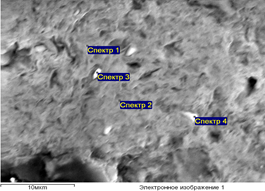
\includegraphics[width=\textwidth]{assets/1043}
        \caption*{а}
    \end{subfigure}
    \hfill
    \begin{subfigure}[b]{0.45\textwidth}
        \centering
        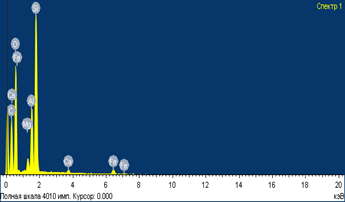
\includegraphics[width=\textwidth]{assets/1043.1}
        \caption*{ә}
    \end{subfigure}
\end{figure}

\begin{table}[H]
\centering
\begin{tabular}{|l|l|l|l|l|l|l|l|l|l|}
\hline
Спектр & Стат. & O & Mg & Al & Si & Ca & Ti & Fe & Қорытынды \\ \hline
1-спектр & Иә & 60.89 & 0.74 & 3.54 & 12.15 & 0.45 & 20.72 & 1.51 & 100.00 \\ \hline
2-спектр & Иә & 63.25 & 0.71 & 3.42 & 30.12 & 0.38 & 0.28 & 1.84 & 100.00 \\ \hline
3-спектр & Иә & 62,41 & 0.59 & 2,68 & 32.84 & 0.41 &  & 01.07 & 100.00 \\ \hline
4-спектр & Иә & 62.68 & 0.44 & 2.,38 & 33.65 &  &  & 0.85 & 100.00 \\ \hline
5-спектр & Иә & 56.65 & 1.95 & 9.28 & 26.86 & 0.92 & 0.45 & 3.89 & 100.00 \\ \hline
Макс. &  & 63.25 & 1.95 & 9.28 & 32.84 & 0.92 & 20.72 & 3.89 &  \\ \hline
Мин. &  & 56.65 & 0.44 & 2.,38 & 12.15 & 0.41 & 0.28 & 0.85 &  \\ \hline
\end{tabular}
\caption*{б}
\caption*{1-сурет - Бентониттің табиғи түрінің микроқұрылымы (а), энергодисперсиондық спектрі (ә), элементтік талдауы (б)}
\end{table}

\begin{multicols}{2}
Электрондық микроскопия бентониттің микросуреттері арқылы кеуек құрылымы
туралы сапалы ақпарат береді, дегенмен кейбір сандық ақпаратты да алуға
болады.

INCA Energy микроталдау жүйесі бар электрондық растрлы микроскоп
көмегімен Таған кен орнының14 көкжиегінің табиғи түрінің микроқұрылымы
зерттелген (1-сур.)

Бентониттердің сорбциялық белсенділігі оларды модификациялау кезінде
жақсарады\emph{.}

\emph{Бентонитті термиялық белсендендіру.} Монтмориллонитті қыздырған
кезде оның суды жоғалтатыны белгілі, бірақ әртүрлі температурада бұл
процесс басқаша жүреді. Әртүрлі кен орындарындағы бентониттердің
сусыздануы олардың түзілу ерекшеліктерімен анықталатын минералогиялық
сипаттамаларына айтарлықтай байланысты {[}4{]}.

Бентониттегі су әртүрлі формада болады: құрылымдық су, адсорбцияланған
су және капиллярлық немесе бос су {[}5{]}. Құрылымдық су немесе
гидроксил түрінде минералдардың құрылымының бөлігі болып табылады және
қатты фазаны 350°C-тан төмен температурада бөлінбейді. Адсорбцияланған
су ішкі және сыртқы беттерде адсорбцияланатын суға сәйкес келеді, яғни
олар агрегаттардың араларындағы кеуектерде (микрокеуектерде) сақталады.
Капиллярлық немесе бос су макрокеуектерде сақталады (2-сур.).
\end{multicols}

\begin{figure}[H]
	\centering
	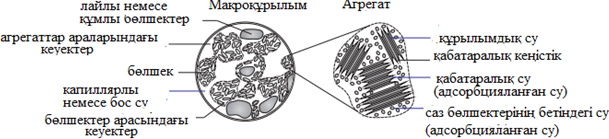
\includegraphics[width=\textwidth]{assets/1044}
	\caption*{2-сурет - Бентонит құрылымының концептуалды бейнесі және әртүрлі суды сақтау механизмдері}
\end{figure}

Бентонитті термиялық белсендендіру 200 \textsuperscript{0}С
температурада жүргізілді.

Термиялық жолмен белсендірілген бентонит сазының электрондық
микроскоппен алынған құырылымдық талдауының нәтижелері 3-суретте
келтірілген.

\begin{figure}[H]
    \centering
    \begin{subfigure}[b]{0.45\textwidth}
        \centering
        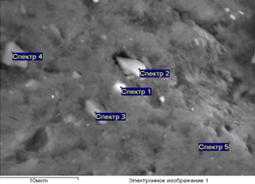
\includegraphics[width=\textwidth]{assets/1045}
        \caption*{а}
    \end{subfigure}
    \hfill
    \begin{subfigure}[b]{0.45\textwidth}
        \centering
        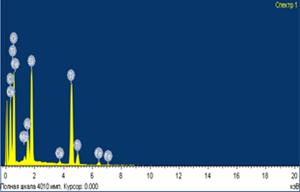
\includegraphics[width=\textwidth]{assets/1045.1}
        \caption*{ә}
    \end{subfigure}
\end{figure}

\begin{table}[H]
\centering
\begin{tabular}{|l|l|l|l|l|l|l|l|l|l|}
\hline
Спектр & Стат. & O & Mg & Al & Si & Ca & Ti & Fe & Қорытынды \\ \hline
1-спектр & Иә & 56.96 & 2.78 & 9.85 & 26.87 & 0.69 &  & 2.85 & 100.00 \\ \hline
2-спектр & Иә & 57.81 & 02.05 & 9.63 & 25.86 & 0.87 &  & 3.78 & 100.00 \\ \hline
3-спектр & Иә & 60.05 & 1.88 & 6.97 & 18.79 & 0.65 & 9.65 & 02.01 & 100.00 \\ \hline
4-спектр & Иә & 63.23 & 1.73 & 4.36 & 28.01 & 0.80 &  & 1,87 & 100.00 \\ \hline
Макс. &  & 63.23 & 2.78 & 9.85 & 28.01 & 0.87 & 9.65 & 3.78 &  \\ \hline
Мин. &  & 56.96 & 1.73 & 4.36 & 18.86 & 0.65 & 9.65 & 1,87 &  \\ \hline
\end{tabular}
\caption*{б}
\caption*{3-сурет - Термиялық жолмен белсендірілген бентониттің микроқұрылымы (а), энергодисперсиондық спектрі (ә) және элементтік талдау (б) нәтижелері}
\end{table}

\begin{multicols}{2}
Термобелсендендірілген бентониттің микроқұрылымы өзгергені көрініп тұр.
Өңделген бентониттің беткі жағы бұдырлы бетке өзгеріп, кеуектілігі
артқан (3-сурет).

Сазды белсендіру температурасы оның адсорбциялық қасиеттеріне әсер
ететіні көрсетілген {[}6{]}.

Сазды 200\textsuperscript{0}С дейін температурада өңдегенде
коллиодтардың бетінен әлсіз байланысқан су бөлініп, саздың бетіндегі
энергетикалық орталықтар босайды да, саздың адсорбциялық қасиеттері
жақсарады. Саздың құрылымы бұл кезде өзгермейді.

Одан жоғары температурада (t\textgreater400°С) өңдеу саздың құрылымын
өзгертіп, коллоидтың энергетикалық белсенділігін төмендетеді. Сондықтан
саздардың адсорбциялық белсенділігі бірнеше есе төмендейді.

Нәтижесінде қабаттардың арасындағы су бөлініп, бентонит бөлшектері мен
кварц түйірлері арасында қашықтық азаяды, электростатикалық тартылыс
күштері артып, бентонит бөлшектерінің бағытталуын жақсартады.

Термиялық өңдеу бентониттің ортасынан бос және құрылымдық суды жойып,
қыздырудың бастапқы кезінде кеуектерді түзеді. Бірақ одан ары қарай
температураны арттыру және уақытын көбейту бентониттің құрылымының
жойылуына және оның беткі ауданын азайтуға әкелуі мүмкін.

Термиялық белсендендіру кезінде кварцтың мөлшері артатыны анықталған
{[}7{]}. Ол бентонит құрамынан қоспалардың және судың бөлінуінен
байқалуы тиіс. Бұл қыздыру кезінде саздан кварцты жоюға болмайтынын
көрсетеді.

Үлгілерді белсендендірудің алдында қатты қыздыру құрылымдық
параметрлерінің біршама өзгеруіне әкеледі. Бұл дегидратация, бентониттің
дисперстлігі, меншікті бетінің өсуімен байланысты. Мүмкін, сазда
температураның және ылғалдың әсерінен саздағы «бітелген кеуектердің» бір
бөлігі ашылып, жеке бөлімдері бұзылып, бір-бірімен жанасатын кеуектердің
жалпы жүйесіне ендіріледі.

Химиялық өңдеу құрылымының өзгеруіне, алмасатын катиондардың құрамы
өзгеруіне және жаңа белсенді орталықтардың пайда болуына байланысты
ионалмасу қасиеттерінің артуына әкеледі. Бентонитті белсендендіру
әдісінің бірі ол жоғары температурадағы қышқылдық белсендендіру болып
табылады.

Термоқышқылдық белсендендіруді өткен бентониттің құрылымдық талдау
нәтижелері 4-суретте көрсетілген.
\end{multicols}

\begin{figure}[H]
    \centering
    \begin{subfigure}[b]{0.45\textwidth}
        \centering
        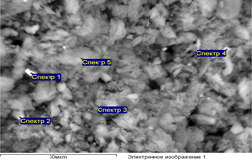
\includegraphics[width=\textwidth]{assets/1046}
        \caption*{а}
    \end{subfigure}
    \hfill
    \begin{subfigure}[b]{0.45\textwidth}
        \centering
        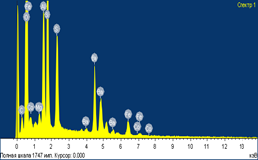
\includegraphics[width=\textwidth]{assets/1046.1}
        \caption*{ә}
    \end{subfigure}
\end{figure}

\begin{table}[H]
\centering
\resizebox{\textwidth}{!}{%
\begin{tabular}{|l|l|l|l|l|l|l|l|l|l|l|l|l|l|}
\hline
Спектр & Стат. & O & Na & Mg & Al & Si & S & Cl & Ca & Ti & Fe & Ba & Қорытынды \\ \hline
1-спектр & Иә & 50.42 &  & 0.84 & 8,97 & 17.37 & 4.56 &  &  &  & 2.44 & 15.4 & 100.00 \\ \hline
1-спектр & Иә & 62.09 &  & 1.10 & 06.05 & 11.52 &  &  & 0.19 & 14.0 & 05.05 &  & 100.00 \\ \hline
1-спектр & Иә & 61.22 & 0.31 & 1.15 & 09.09 & 23.47 &  & 0.15 & 0.21 & 0.35 & 04.05 &  & 100.00 \\ \hline
1-спектр & Иә & 63.77 & 0.67 & 0.74 & 7.26 & 24.71 &  &  & 0.15 & 0.25 & 2.45 &  & 100.00 \\ \hline
1-спектр & Иә & 64.41 & 0.57 & 0.84 & 6.56 & 25.09 &  & 0.16 & 0.29 &  & 02.08 &  & 100.00 \\ \hline
Макс. &  & 64.41 & 0.67 & 1.15 & 09.09 & 25.09 & 4.56 & 0.16 & 0.22 & 14.0 & 05.05 & 15.4 &  \\ \hline
Мин. &  & 50.42 & 0.31 & 0.74 & 6.56 & 11.50 & 4.56 & 0.15 & 0.15 & 0.25 & 02.08 & 15.4 &  \\ \hline
\end{tabular}
}
\caption*{б}
\caption*{4-сурет - Термоқышқылдық жолмен белсендендірілген бентониттің микроқұрылымы (а), энергодисперсиондық спектрі (ә), элементтік талдау (б) нәтижелері}
\end{table}

\begin{multicols}{2}
Термоқышқылдық әдіспен белсендірілген түрінде бентониттің
микроқұрылымының елеулі өзгергені, беті бос, кеуекті және қабыршақты
болатыны көрінеді.

Бентонитті қышқылдық белсендіру үлгідегі магний, темір, сілтілі және
сілтілікжер металдардың оксидтері мөлшерінің азаюуына әкеледі, себебі
бұл процесс кезінде металдардың оксидтері шайылады.

Бентониттерді қышқылдық белсендіру кезінде \emph{Na\textsuperscript{+},
K\textsuperscript{+}, Ca\textsuperscript{2+}, Mg\textsuperscript{2+}}
иондарын сутек иондарына алмастырудан басқа монтмориллониттің кристалдық
құрылымы бұзылады. Алмасуға қабілетті \emph{Н\textsuperscript{+}} және
\emph{Al\textsuperscript{3+ }}катиондары түзіледі және алмасатын
алюминий катиондары сутек катиондарынан көбірек болады.

Термоқышқылды белсендіру кезінде сілтілікжер металдардың иондарын
ығыстыратын ион - сутек катионы H\textsuperscript{+} болады. Сулы ортада
ең аз мөлшеріне байланысты ең үлкен қозғалғыштығы бар ион алмасу
процесінде протон кальций мен магний иондарының қосымша мөлшерін
жылжымалы түрге айналдыра отырып, материалдың ион алмасу қабілетін
барынша арттыруы тиіс {[}8{]}.

Бентонит саздарын қышқылдық активтендіру кезінде тек октаэдрлік
(орталық) қабаты ғана емес, монтмориллонит торының тетраэдрлік қабаттары
да бұзылады. Бұл тетраэдрлік

және октаэдрлік қабаттардағы изоморфты алмастырулар санының азаюымен
дәлелденеді.

Монтмориллонит құрылымынан алынған алюминий иондарының қалған бөлігі
магний мен темір иондарын алмасу орындарынан ығыстырып, оның теріс
зарядтарының орнын толтыру үшін тормен байланысады және
Н\textsuperscript{+} иондарымен бірге алмасатын қышқылдығын
(H\textsuperscript{+}+Al\textsuperscript{3+}) негіздейді.

\emph{Бентонитті қолдана отырып ағынды суларды тазарту.}

Зерттеуге алынған Шығыс-Қазақстан облысындағы Белоус полиметалл кен
орынының шахта суларының сипаттамасы төменде 3-кестеде келтірілген.
\end{multicols}

\begin{figure}[H]
    \centering
    \begin{subfigure}[b]{0.45\textwidth}
        \centering
        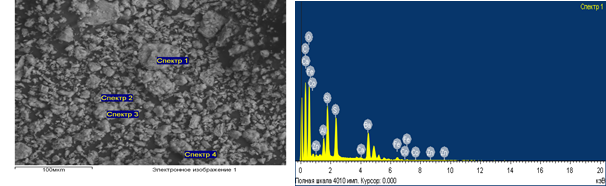
\includegraphics[width=\textwidth]{assets/1048}
        \caption*{а}
    \end{subfigure}
    \hfill
    \begin{subfigure}[b]{0.45\textwidth}
        \centering
        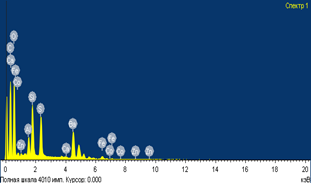
\includegraphics[width=\textwidth]{assets/1048.1}
        \caption*{ә}
    \end{subfigure}
\end{figure}

\begin{table}[H]
\centering
\resizebox{\textwidth}{!}{%
\begin{tabular}{|l|l|l|l|l|l|l|l|l|l|l|l|l|l|}
\hline
Спектр & Стат. & О & Mg & Al & Si & S & Ca & Ti & Fe & Zn & Co & Ba & Қорытынды \\ \hline
1-спектр & Иә & 42.03 &  & 5.35 & 10.57 & 5.42 & 0.38 &  & 02.06 & 11.02 & 0.0 & 23.14 & 100.00 \\ \hline
2-спектр & Иә & 56.97 & 0.76 & 5.54 & 10.99 &  & 0.66 & 21.77 & 3.31 &  &  &  & 100.00 \\ \hline
3-спектр & Иә & 43.56 & 0.88 & 3.82 & 16.00 &  & 0.56 &  & 35.18 &  &  &  & 100.00 \\ \hline
4-спектр & Иә & 54.86 & 1.85 & 10.96 & 25.76 &  & 0.87 & 0.72 & 4.98 &  &  &  & 100.00 \\ \hline
5-спектр & Иә & 55.65 & 1.49 & 10.49 & 26.88 &  & 0.80 &  & 4.69 &  &  &  & 100.00 \\ \hline
Макс. &  & 56.97 & 1.85 & 10.96 & 26.88 & 5.42 & 0.87 & 21.77 & 35.18 & 11.02 & 0.0 & 23.14 &  \\ \hline
Мин. &  & 42.06 & 0.76 & 3.82 & 10.57 & 5.42 & 0.38 & 0.72 & 02.06 & 11.02 & 0.0 & 23.14 &  \\ \hline
\end{tabular}
}
\caption*{Барлық нәтижелер массалық \%}
\caption*{5-сурет - Термоқышқылдық жолмен белсендірілген бентонит сазының микроқұрылымы (а), энергодисперсиондық спектрі (ә), элементтік талдау нәтижелері (в) ағынды сумен әрекеттескеннен кейін}
\end{table}

\begin{table}[H]
\caption*{3-кесте - Шығыс-Қазақстан облысындағы Белоус полиметалл кен орынының шахта суларының сипаттамасы (рН 7,1÷7,6)}
\centering
\begin{tabular}{|l|ll|}
\hline
\multirow{2}{*}{Компоненттер} & \multicolumn{2}{l|}{Компоненттің мөлшері, мг/дм$^{3}$} \\ \cline{2-3}
 & \multicolumn{1}{l|}{тұнбада} & фильтратта \\ \hline
Cu$^{2+}$ & \multicolumn{1}{l|}{8,20$\pm$0,20} & 0,21$\pm$0,04 \\ \hline
Pb$^{2}$ & \multicolumn{1}{l|}{4,80$\pm$0,16} & 0,11$\pm$0,03 \\ \hline
Cd$^{2+}$ & \multicolumn{1}{l|}{0,25$\pm$0,02} & 0,17$\pm$0,02 \\ \hline
Zn$^{2+}$ & \multicolumn{1}{l|}{67,10$\pm$0,63} & 12,3$\pm$0,39 \\ \hline
Жүзгін заттар & \multicolumn{1}{l|}{260} & 50 \\ \hline
\end{tabular}
\end{table}

\begin{multicols}{2}
Ауыр металдардың сазбен сорбциялануы негізінен екі механизм арқылы
жүреді: ион алмасу (монтмориллониттің қабат аралық кеңістіктерінде
орналасқан катиондардың алмасуы) және минералдың беткі гидроксил
топтарымен хелаттық кешендердің түзілуі. Табиғи минералдың құрамына
байланысты сорбция процесінің механизмі әртүрлі болуы мүмкін {[}9-11{]}.

Ион алмасумен қатар бентонит саздарында физикалық және молекулалық
сорбция жүруі мүмкін. Физикалық сорбция иондануға қабілетті қышқылдық
және негіздік сипаттағы кристалдық беттер мен беттік гидроксид
топтарында артық теріс зарядтың болуына байланысты.

Молекулалық сорбция кезінде қабаттар арасында сорбцияланған заттар
орналасады, қабаттардың құрылымын өзгертпейді. Осылайша, мұндай белсенді
орталықтар - алмасатын катиондары, гидроксил топтары, бентонит
саздарының активтенуі осы сорбенттердің практикалық қолданысын
арттырады.

Термоқышқылдық жолмен белсендірілген бентонит сазының ағынды сумен
жанасқаннан кейін құрамында сілтілі және сілтілі жер металдарының
катиондары ғана емес, сонымен қатар, құрамындағы қоспалар да бар, майда
кристалды құрылымы бар тығыз материал түзіледі (5-сурет). Көрсетілген
нәтиже мырыш элементінің бар екендігін көрсетеді. Бұл термоқышқылды
жолмен белсендірілген түрдегі бентониттің ағынды сумен байланысқаннан
кейін мырыш иондарының сорбцияланғанын дәлелдейді.

Ағынды суларды ауыр металдар иондарынан (\emph{Cu\textsuperscript{2+},
Pb\textsuperscript{2+}, Cd\textsuperscript{2+}, Zn\textsuperscript{2+}})
бентониттің түрлі формаларымен тазарту нәтижелерін салыстыру төмендегі
4-кестеде келтірілген.
\end{multicols}

\begin{table}[H]
\caption*{4-кесте - Табиғи және термиялық қышқылмен белсендірілген бентонитті пайдалана отырып, шахта суынан ауыр металл иондарын алу}
\centering
\begin{tabular}{|p{0.15\textwidth}|lllp{0.15\textwidth}|}
\hline
\multirow{3}{=}{Металдардың иондары} & \multicolumn{4}{l|}{Бентонит} \\ \cline{2-5}
 & \multicolumn{4}{l|}{Иондырдың сіңірілуі, \%} \\ \cline{2-5}
 & \multicolumn{1}{l|}{табиғи} & \multicolumn{1}{p{0.15\textwidth}|}{қышқылмен белсендірілген} & \multicolumn{1}{p{0.15\textwidth}|}{термиялық жолмен белсендірілген} & термоқышқылды жолмен белсендірілген \\ \hline
Cu$^{2+}$ & \multicolumn{1}{l|}{15,1} & \multicolumn{1}{l|}{16,2} & \multicolumn{1}{l|}{25,7} & 96,4 \\ \hline
Pb$^{2+}$ & \multicolumn{1}{l|}{78,7} & \multicolumn{1}{l|}{91,4} & \multicolumn{1}{l|}{83,5} & 98,2 \\ \hline
Cd$^{2+}$ & \multicolumn{1}{l|}{26,2} & \multicolumn{1}{l|}{48,7} & \multicolumn{1}{l|}{39,5} & 94,1 \\ \hline
Zn$^{2+}$ & \multicolumn{1}{l|}{96,3} & \multicolumn{1}{l|}{34,8} & \multicolumn{1}{l|}{97,2} & \multicolumn{1}{r|}{98,6} \\ \hline
\end{tabular}
\end{table}

\begin{multicols}{2}
Алынған нәтижелерден көрініп тұрғандай, қышқылдық активтенуден өткен
бентонит сазын алдын ала термиялық өңдеусіз қолданғанда, ауыр металдар
иондарының экстракциялану дәрежесі термиялық активтендірілген немесе
термоқышқылды белсендірілген формаларды пайдаланғанға қарағанда төмен
(4-кесте). Мұның себептері пайдаланылған үлгінің ісінуіне байланысты
болуы, сонымен қатар, зерттелетін катиондар ғана емес, басқа да полярлы
органикалық және бейорганикалық қосылыстардың молекулалары ауыр металдар
иондарымен бәсекелесіп, аралық кеңістікке еніп кетуі мүмкіндігіне
байланысты.

Шахта суын тазартуда термиялық және қышқылмен белсендірілген бентонитті
(200 \textsuperscript{0}С температурада -4 сағат, содан кейін 4 сағат
бойы 10\% H\textsubscript{2}SO\textsubscript{4} өңдеу) пайдалану ауыр
металдары иондарының толықтай дерлік экстракциялануын қамтамасыз етеді
Cu\textsuperscript{2+}, Pb\textsuperscript{2+}, Cd\textsuperscript{2+},
Zn\textsuperscript{2+} (сәйкес 96,4 ; 98,2; 94,1; 98,6\%).
\end{multicols}

\begin{table}[H]
\caption*{5-кесте - Түрлі бентонит формаларымен тазартылған ағынды судағы ауыр металдар иондарының концентрациясы}
\centering
\begin{tabular}{|p{0.15\textwidth}|llllp{0.15\textwidth}|}
\hline
\multirow{3}{=}{Металдардың иондары} & \multicolumn{5}{l|}{Ауыр металдар иондарының концентрациясы, мг/дм$^{3}$} \\ \cline{2-6}
 & \multicolumn{1}{p{0.15\textwidth}|}{\multirow{2}{=}{Тазартылмаған суда, С}} & \multicolumn{1}{l|}{\multirow{2}{*}{ШРК\tsb{б-ш.}}} & \multicolumn{3}{l|}{Тазартылған шахта суында} \\ \cline{4-6}
 & \multicolumn{1}{l|}{} & \multicolumn{1}{l|}{} & \multicolumn{1}{p{0.15\textwidth}|}{табиғи  бентонитпен, С\tsb{б}} & \multicolumn{1}{p{0.15\textwidth}|}{термиялық белсендірілген бентонитпен, С\tsb{т}} & термоқышқылды белсендірілген бентонитпен, С\tsb{тқ} \\ \hline
Cu$^{2+}$ & \multicolumn{1}{l|}{0,21} & \multicolumn{1}{l|}{0,001} & \multicolumn{1}{l|}{0,1} & \multicolumn{1}{l|}{0,07} & 0,001 \\ \hline
Pb$^{2+}$ & \multicolumn{1}{l|}{0,11} & \multicolumn{1}{l|}{0,1} & \multicolumn{1}{l|}{0,09} & \multicolumn{1}{l|}{0,03} & 0,01 \\ \hline
Cd$^{2+}$ & \multicolumn{1}{l|}{0,17} & \multicolumn{1}{l|}{0,005} & \multicolumn{1}{l|}{0,14} & \multicolumn{1}{l|}{0,09} & 0,006 \\ \hline
Zn$^{2+}$ & \multicolumn{1}{l|}{12,3} & \multicolumn{1}{l|}{0,01} & \multicolumn{1}{l|}{8,7} & \multicolumn{1}{l|}{4,03} & 0,01 \\ \hline
\end{tabular}
\end{table}

\begin{multicols}{2}
6-кестеде әртүрлі формадағы бентонит сазымен ағынды сулардан ауыр
металдар иондарын сорбциялау нәтижелері: табиғи, термикалық
белсендірілген, термиялық қышқылмен белсендірілген, сондай-ақ олардың
бастапқы, тазартылған ағынды сулардың концентрациясының қатынасы ретінде
салыстырмалы деректері келтірілген.
\end{multicols}

\begin{table}[H]
\caption*{6-кесте - Шаруашылық қызмет үшін судағы осы иондардың шекті рұқсат етілген концентрацияларымен (ШРК) салыстырғанда ауыр металл иондарын бентонит сазымен сіңіру}
\centering
\resizebox{\textwidth}{!}{%
\begin{tabular}{|p{0.15\textwidth}|llllll|}
\hline
\multirow{3}{=}{Ауыр металл иондарының концентрациясы} & \multicolumn{6}{l|}{Ауыр металл иондарының концентрациясы, мг/дм\tsp{3}} \\ \cline{2-7}
 & \multicolumn{1}{p{0.15\textwidth}|}{\multirow{2}{=}{тазартылмаған суда, С\tsb{0}}} & \multicolumn{1}{l|}{\multirow{2}{*}{ШРК\tsb{б-ш.}}} & \multicolumn{1}{l|}{\multirow{2}{*}{С\tsb{0}/ШРК\tsb{б-ш.}}} & \multicolumn{3}{p{0.4\textwidth}|}{Ауыр металдар иондарының концентрациясының тазартылғаннан кейін ШРКб-ш. қатынасы} \\ \cline{5-7}
 & \multicolumn{1}{l|}{} & \multicolumn{1}{l|}{} & \multicolumn{1}{l|}{} & \multicolumn{1}{l|}{С\tsb{и}/ШРК\tsb{б-ш.}} & \multicolumn{1}{l|}{С\tsb{т} /ШРК\tsb{б.-ш.}} & Стк/ ШРКб-ш. \\ \hline
Cu$^{2+}$ & \multicolumn{1}{l|}{0,21} & \multicolumn{1}{l|}{0,001} & \multicolumn{1}{l|}{210} & \multicolumn{1}{l|}{140} & \multicolumn{1}{l|}{70} & 1 \\ \hline
Pb$^{2+}$ & \multicolumn{1}{l|}{0,11} & \multicolumn{1}{l|}{0,1} & \multicolumn{1}{l|}{1,1} & \multicolumn{1}{l|}{0,9} & \multicolumn{1}{l|}{0,3} & 0,1 \\ \hline
Cd$^{2+}$ & \multicolumn{1}{l|}{0,17} & \multicolumn{1}{l|}{0,005} & \multicolumn{1}{l|}{34} & \multicolumn{1}{l|}{38} & \multicolumn{1}{l|}{4,5} & 1,2 \\ \hline
Zn$^{2+}$ & \multicolumn{1}{l|}{12,3} & \multicolumn{1}{l|}{0,01} & \multicolumn{1}{l|}{1230} & \multicolumn{1}{l|}{870} & \multicolumn{1}{l|}{40,3} & 1 \\ \hline
\end{tabular}
}
\end{table}

\begin{multicols}{2}
Берілген арақатынастарды С\textsubscript{б}/ШРК\textsubscript{б.-ш.,}
С\textsubscript{т}/ШРК\textsubscript{б.-ш.,}
С\textsubscript{тк}/ШРК\textsubscript{б.-ш.,} ауыр металдарды саздың әр
түрлі формалары: табиғи, термиялық және термоқышқылдық жолмен
белсендірілген бентонитті қолданғанда, зерттелетін иондарға қатысты ең
жақсы сорбент термоқышқылды белсендірілген бентонит екенін көрсетеді.

7-кестеде зерттеу нәтижелерінің метрологиялық сипаттамалары берілген.
\end{multicols}

\begin{table}[H]
\caption*{7-кесте - Зерттеу нәтижелерін метрологиялық бағалау (конвергенция, қайталану және дәлдіктің стандартты ауытқуы)}
\centering
\begin{tabular}{|l|l|l|l|}
\hline
Ауыр металдардың иондары & S\tsb{сх.} ·104 & S\tsb{қайт.} ·104 & S\tsb{дұр.} ·104 \\ \hline
Cu$^{2+}$ & 1,81 & 2,95 & 1,25 \\ \hline
Cd$^{2+}$ & 1,92 & 2,89 & 2,52 \\ \hline
Pb$^{2+}$ & 2,69 & 5,35 & 1,83 \\ \hline
Zn$^{2+}$ & 15,9 & 25,3 & 23,5 \\ \hline
\end{tabular}
\end{table}

\begin{multicols}{2}
Алынған зерттеу нәтижелері бойынша есептелген метрологиялық сипаттамалар
(қайталанудың стандартты ауытқуларының мәні, нәтижелердің
дұрыстығын/дәлдігін бақылау) (7 кесте) зерттелетін барлық металл иондары
(Cu\textsuperscript{2+}, Cd\textsuperscript{2+}, Pb\textsuperscript{2+},
Zn\textsuperscript{2+}) үшін жүйелі қателер бойынша статистикалық
маңызды емес.

{\bfseries Қорытынды.} Эксперименттік зерттеулер нәтижесі бойынша:

- Шығыс Қазақстан облысындағы Белоусов полиметалл кен орнының шахта
суларынан ауыр металл иондарының Шығыс Қазақстан облысы Таған кен
орнының 14 горизонтындағы үш түрлі модификацияда: табиғи, қышқылды
активтендірілген және термоқышқылды белсендірілген бентонит сазымен
адсорбциясы туралы мәліметтер алынды;

- бастапқы ағынды сулардың концентрациясының тазартылған ағынды суларға
қатынасы шекті рұқсат етілген концентрация мәндерімен салыстыра
зерттелді;

- зерттелетін иондарға қатысты ең тиімді сорбент бентонит сазының
термоқышқылды белсендірілген түрі болатыны анықталды;

- бірқатар тәжірибелер негізінде оңтайлы жағдайларда термоқышқылды
жолмен белсендірілген бентонит сазы ағынды сулардан
Cu\textsuperscript{2+}, Pb\textsuperscript{2+}, Cd\textsuperscript{2+},
Zn\textsuperscript{2+} иондарын тиісінше 99,6, 94,7, 98,9 және 99,5\%-ға
жоюға, мүмкіндік беретіні анықталды. Бұл балық шаруашылығы үшін арналған
суларға шектеулі рұқсат етілген концентрациялары мәндеріне сәйкес
келеді.

\emph{{\bfseries Қаржыландыру}.} Бұл ғылыми зерттеу IRN AP19674742 «Шығыс
Қазақстанның табиғи бентониті негізінде жаңа органикалық минералды
композициялық материалды алу технологиясы» жобасын гранттық қаржыландыру
шеңберінде жүзеге асырылды. Қаржыландыру көзі -- Қазақстан Республикасы
Ғылым және жоғары білім министрлігінің Ғылым комитеті.
\end{multicols}
\newpage
\begin{center}
{\bfseries Әдебиеттер}
\end{center}

\begin{noparindent}
1.Сапаргалиев Е.М. Влияние вещественного состава сырья на
технологические свойства бентонитов Таганского месторождения //Вестник
РУДН. Серия инженерные исследования. - 2007. -№2. -C. 77-81

2. Shamkhanov M.Ch. Adsorbenty na osnove prirodnogo bentonita //Vestnik
magistratury. -2021. -№ 5 (116). -S. 34-37

3. Dieudonne A.C. Microstructure of bentonites: characterisation and
evolution under mechanical and environmental loads //EURAD School for
Radioactive Waste Management. Belgium. -2020, -P. 1-21.

4. Горюшкин В.В. Технологические свойства бентонитов палеоцена
воронежской антеклизы и возможности их изменения // Вестник воронежского
университета. Геология. -2005. -№ 1. -C. 166-177

5.Jacinto A. C., Villar, Ledesma M. V. Influence of water density on the
water-retention curve of expansive clays// Geotechnique. -2012. -№
8(62). -P. 657-667.

6.Анюхина А.В., Середин В.В., Андрианов А.В., Хлуденева Т.Ю. Влияние
термической обработки глин на их адсорбцию по красителю метиленовый
голубой // Недропользование. -2021. -Т. 21. -№ 2. -С.52-57. DOI
10.15593/2712-8008/2021.2.1

7.Amari A., Chlendi M., Gannouni A., Bellagi A. Optimised activation of
bentonite for toluene adsorption // Applied Clay Science. -2010. -№47.
--P:447-461

8.Burakov A.E., Galunin EV, Burakova IV, Kucherova AE, Agarwal S,
Tkachev A.G., Gupta V.K. Adsorption of heavy metals on conventional and
nanostructured materials for wastewater treatment purposes: A review//
Ecotoxicology and Environmental Safety. -2018.-№148, -P.702--712. DOI
10.1016/j.ecoenv.2017.11.034.

9.Кошелев А. В., Веденеева Н. В., Заматырина В. А., Тихомирова Е. И.,
Скиданов Е. В. Разработка технологии получения сорбентов на основе
бентонитовых глин для систем очистки воды // Вода и экология: проблемы и
решения. -2018. -№ 2 (74), - C. 32-39 DOI
10.23968/2305--3488.2018.20.2.32--39

10. Bourliva A., Michailidis K, Sikalidis C, Filippidis A, Betsiou M.
Adsorption of Cd(II), Cu(II), Ni(II) and Pb(II) on to natural bentonite:
study in mono- and multi- metal systems // Environ Earth Sci. - 2015.
--Vol. 73. --P. 5435--5444. DOI 10.1007/s12665-014-3798-0 11.Черкасов
А.С., Сомин В.А., Комарова Л.Ф., Куртукова Л.В. Изучение сорбционных
свойств бентонита милосского месторождения и материала на его основе //
Ползуновский вестник. - 2014. - №3. с. 254-256
\end{noparindent}

\begin{center}
{\bfseries References}
\end{center}

\begin{noparindent}
1. Sapargaliev E.M. Vliyanie veshchestvennogo sostava
syr\textquotesingle ya na tekhnologicheskie svoistva bentonitov
Taganskogo mestorozhdeniya //Vestnik RUDN. Seriya inzhenernye
issledovaniya. - 2007. -№2. -S. 77-81 {[}in Russian{]}

2. Shamkhanov M.Ch. Adsorbenty na osnove prirodnogo bentonita //Vestnik
magistratury.//-2021. -№ 5 (116). -S. 34-37. {[}in Russian{]}

3. Dieudonne A.C. Microstructure of bentonites: characterisation and
evolution under mechanical and environmental loads //EURAD School for
Radioactive Waste Management. Belgium. -2020, -P. 1-21

4. Goryushkin V.V. Tekhnologicheskie svoistva bentonitov paleotsena
voronezhskoi anteklizy i vozmozhnosti ikh izmeneniya // Vestnik
voronezhskogo universiteta. Geologiya. -2005. -№ 1. -S. 166-177. {[}in
Russian{]}

5. Jacinto A. C., Villar, Ledesma M. V. Influence of water density on
the water-retention curve of expansive clays// Geotechnique. -2012. -№
8(62). -P. 657-667.

6. Anyukhina A.V., Seredin V.V., Andrianov A.V., Khludeneva T.Yu.
Vliyanie termicheskoi obrabotki glin na ikh adsorbtsiyu po krasitelyu
metilenovyi goluboi // Nedropol\textquotesingle zovanie. -2021. -T. 21.
-№ 2, -S.52-57. DOI 10.15593/2712-8008/2021.2.1 {[}in Russian{]}

7. Amari A., Chlendi M., Gannouni A., Bellagi A. Optimised activation of
bentonite for toluene adsorption // Applied Clay Science. -2010. -№47.
--P:447-461

8. Burakov A.E., Galunin EV, Burakova IV, Kucherova AE, Agarwal S,
Tkachev A.G., Gupta V.K. Adsorption of heavy metals on conventional and
nanostructured materials for wastewater treatment purposes: A review//
Ecotoxicology and Environmental Safety. -2018. -№148. -P.702--712. DOI
10.1016/j.ecoenv.2017.11.034.

9. Koshelev A. V., Vedeneeva N. V., Zamatyrina V. A., Tikhomirova E. I.,
Skidanov E. V. Razrabotka tekhnologii polucheniya sorbentov na osnove
bentonitovykh glin dlya sistem ochistki vody // Voda i ehkologiya:
problemy i resheniya. -2018. -№ 2 (74), - S.32-39 DOI
10.23968/2305--3488.2018.20.2.32--39 {[}in Russian{]}

10. Bourliva A., Michailidis K, Sikalidis C, Filippidis A, Betsiou M.
Adsorption of Cd(II), Cu(II), Ni(II) and Pb(II) on to natural bentonite:
study in mono- and multi- metal systems // Environ Earth Sci. - 2015.
--Vol. 73. --P. 5435--5444. DOI 10.1007/s12665-014-3798-0

11. Cherkasov A.S., Somin V.A., Komarova L.F., Kurtukova L.V. Izuchenie
sorbtsionnykh svoistv bentonita milosskogo mestorozhdeniya i materiala
na ego osnove // Polzunovskii vestnik. -2014. - №3. - S. 254-256. {[}in
Russian{]}
\end{noparindent}

\emph{{\bfseries Авторлар туралы мәліметтер}}

\begin{noparindent}
Рожкова О.В. - химия ғылымдарының докторы, профессор, Қазақстан
Республикасы Ұлттық жаратылыстану ғылымдары академиясының академигі,
«Сәкен Сейфуллин атындағы Қазақ агротехникалық зерттеу университеті»
КЕАҚ, Астана, Қазақстан, «Science and Technology Solutions» АҚ, Алматы,
Қазақстан, e-mail:

rozhkova.o@ stsolutions.kz;

Мұздыбаева Ш.А. - химия ғылымдарының кандидаты, Халықаралық
инженерлік-технологиялық университетінің доценті, Алматы қ., Қазақстан,
e-mail: sharbanu1958@mail.ru;

Бөкеева А.Б. - химия ғылымдарының кандидаты, «Қазақ агротехникасы --
химия ғылымдарының кандидаты» КЕАҚ, «Сәкен Сейфуллин атындағы Қазақ
агротехникалық университеті» КЕАҚ, Астана, Қазақстан, e-mail:
akbota712@mail.ru;

Құдайбергенова С.Ж. - химия ғылымдарының кандидаты, «Сәкен Сейфуллин
атындағы Қазақ агротехникалық университеті» КЕАҚ, Астана, Қазақстан,
e-mail: ksg.75.75@mail.ru;

Рожков В.И. - техника ғылымдарының кандидаты, «Сәкен Сейфуллин атындағы
Қазақ агротехникалық университеті» КЕАҚ, Астана, Қазақстан, «Алтай
геологиялық-экологиялық институты» ЖШС, Өскемен, Қазақстан, e-mail:
vitalrza1983@gmail.com;

Ермеков М.Т. - «Ғылым және технологияларды дамыту» АҚ Жоба және
активтерді басқару департаментінің директоры, Алматы, Қазақстан, e-mail:
yermekov.m@stsolutions.kz;

Нұртай Ж.Т. - PhD, Қ.Құлажанов атындағы Қазақ технология және бизнес
университетінің доценті, Астана, Қазақстан, e-mail:
zhadira\_nurtai@mail.ru
\end{noparindent}

\emph{{\bfseries Information about the authors}}

\begin{noparindent}
Rozhkova O.V. - Doctor of chemical sciences, professor, academician of
the National Academy of Natural Sciences of the Republic of Kazakhstan,
NAO ``Kazakh Agrotechnical Research University named after Saken
Seyfullin'', Astana, Kazakhstan, JSC ``Science and Technology
Solutions'', Almaty, Kazakhstan, e-mail:

rozhkova.o@stsolutions.kz;

Muzdybaeva Sh.A. - Candidate of Chemical Sciences, Associate Professor,
``International Engineering and

Technological University'', Almaty,
Kazakhstan, e-mail: sharbanu1958@mail.ru;

Bukeeva A.B. - Candidate of Chemical Sciences, NAO ``Kazakh
Agrotechnical - Candidate of Chemical Sciences, NAO `Kazakh
Agrotechnical University named after Saken Seyfullin', Astana,
Kazakhstan, e-mail:

akbota712@mail.ru;

Kudaibergenova S.Zh. - Candidate of Chemical Sciences, NAO ``Kazakh
Agrotechnical University named after Saken Seifullin'', Astana,
Kazakhstan, e-mail: ksg.75.75@mail.ru;

Rozhkov V.I. - Candidate of Technical Sciences, NAO ``Kazakh
Agrotechnical University named after Saken Seifullin'', Astana,
Kazakhstan, LLP ``Altai Geological and Ecological Institute'',
Ust-Kamenogorsk, Kazakhstan, e-mail: vitalrza1983@gmail.com;

Ermekov M.T. - Director of Projects and Asset Management Department,
``Science and Technology olutions'' JSC, Almaty, Kazakhstan, e-mail:
yermekov.m@stsolutions.kz;

Nurtay J.T. - PhD, Associate Professor, ``Kazakh University of
Technology and Business named after K.Kulazhanov'', Astana, Kazakhstan,
e-mail: zhadira\_nurtai@mail.ru.
\end{noparindent}
